\documentclass{beamer}
\usetheme[sectionpage=progressbar, subsectionpage=progressbar, numbering=fraction, progressbar=foot, block=fill, background=light]{metropolis}
\usepackage{appendixnumberbeamer}
\usepackage{textpos}
\usepackage{booktabs}
\usepackage[scale=2]{ccicons}

\usepackage{pgfplots}
\usepgfplotslibrary{dateplot}
\usetikzlibrary{backgrounds}
\usepackage{xspace}
\newcommand{\themename}{\textbf{\textsc{metropolis}}\xspace}
\title{Attention based models in End-to-End ASR}
\subtitle{Exploration of Attention in ESPNET toolkit}
\date{\today}
\author{Shreekantha Nadig}
\institute{International Institute of Information Technology - Bangalore}
%\titlegraphic{\hfill\includegraphics[height=1.5cm]{logo.pdf}}

\usepackage{tikz}
\usetikzlibrary{shapes,shadows,arrows,patterns}
\tikzstyle{line} = [draw, -latex']
\tikzstyle{round} = [draw, circle, fill=black!30, minimum size=4em, node distance=4em]
\tikzstyle{mlp_enc} = [rectangle, draw, fill=red!50, text width=5em, minimum height=5em, text centered, node distance=10em]
\tikzstyle{mlp_att} = [rectangle, draw, fill=green!50, text width=5em, minimum height=5em, text centered, node distance=10em]
\tikzstyle{mlp_dec} = [rectangle, draw, fill=blue!50, text width=5em, minimum height=5em, text centered, node distance=10em]
\tikzstyle{enc_h} = [rectangle, draw,  pattern=north west lines, pattern color=red!60, text width=1em, minimum height=10em, minimum width=3em, text centered, node distance=10em]
\tikzstyle{atts} = [rectangle, draw,  pattern=north west lines, pattern color=green!70, text width=1em, minimum height=10em, minimum width=3em, text centered, node distance=10em]
\tikzstyle{dec_z} = [rectangle, draw,  pattern=north east lines, pattern color=blue!60, text width=1em, minimum height=10em, minimum width=3em, text centered, node distance=10em]
\begin{document}
\addtobeamertemplate{frametitle}{}{%
	\begin{textblock*}{100mm}(.97\textwidth,-1cm)
		{\includegraphics[width=2.5em]{iiitb_logo.png}}
	\end{textblock*}}
\maketitle

\begin{frame}{Table of contents}
	\setbeamertemplate{section in toc}[sections numbered]
	\tableofcontents[hideallsubsections]
\end{frame}

\section{Introduction}
	\begin{frame}[fragile]{BLSTM}
	\begin{center}
		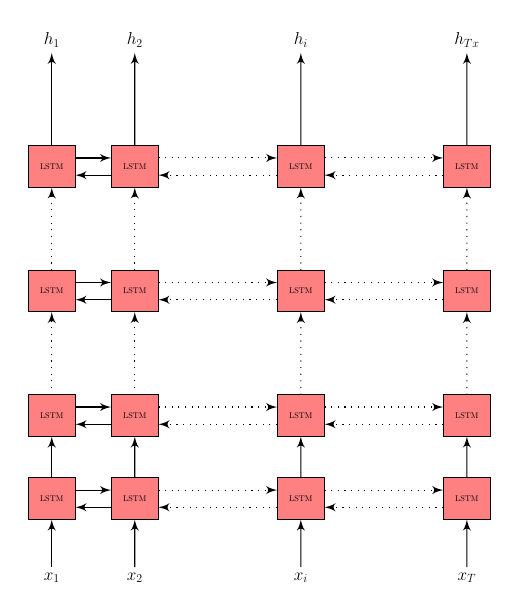
\begin{tikzpicture}[scale=0.3, every node/.style={transform shape}]
		\onslide<1->\node[mlp_enc](LSTM_1_1){LSTM};
		\node[mlp_enc, right of=LSTM_1_1](LSTM_1_2) {LSTM};
		\path [line] (LSTM_1_1.20) to (LSTM_1_1.20-|LSTM_1_2.west);
		\path [line] (LSTM_1_2.200) to (LSTM_1_2.-20-|LSTM_1_1.east);     
		
		\node[mlp_enc, right of=LSTM_1_2, node distance = 20em](LSTM_1_i) {LSTM};
		\path [line, dotted] (LSTM_1_2.20) to (LSTM_1_2.20-|LSTM_1_i.west);
		\path [line, dotted] (LSTM_1_i.200) to (LSTM_1_i.200-|LSTM_1_2.east);
		
		\node[mlp_enc, right of=LSTM_1_i, node distance = 20em](LSTM_1_Tx) {LSTM};
		\path [line, dotted] (LSTM_1_i.20) to (LSTM_1_i.20-|LSTM_1_Tx.west);
		\path [line, dotted] (LSTM_1_Tx.200) to (LSTM_1_Tx.200-|LSTM_1_i.east);
		{\fontsize{20}{11}\selectfont
		\node [below of=LSTM_1_1, node distance = 5em] (x1) {$x_{1}$};
		\node [below of=LSTM_1_2, node distance = 5em] (x2) {$x_{2}$};
		\node [below of=LSTM_1_i, node distance = 5em] (xi) {$x_{i}$};
		\node [below of=LSTM_1_Tx, node distance = 5em] (xTx) {$x_{T}$};
		}
		\path [line] (x1) to (LSTM_1_1);
		\path [line] (x2) to (LSTM_1_2);
		\path [line] (xi) to (LSTM_1_i);
		\path [line] (xTx) to (LSTM_1_Tx);
		
		\onslide<2->\node[mlp_enc, above of = LSTM_1_1](LSTM_2_1){LSTM};
		\node[mlp_enc, right of=LSTM_2_1](LSTM_2_2) {LSTM};
		\path [line] (LSTM_2_1.20) to (LSTM_2_1.20-|LSTM_2_2.west);
		\path [line] (LSTM_2_2.200) to (LSTM_2_2.-20-|LSTM_2_1.east);     
		
		\node[mlp_enc, right of=LSTM_2_2, node distance = 20em](LSTM_2_i) {LSTM};
		\path [line, dotted] (LSTM_2_2.20) to (LSTM_2_2.20-|LSTM_2_i.west);
		\path [line, dotted] (LSTM_2_i.200) to (LSTM_2_i.200-|LSTM_2_2.east);
		
		\node[mlp_enc, right of=LSTM_2_i, node distance = 20em](LSTM_2_Tx) {LSTM};
		\path [line, dotted] (LSTM_2_i.20) to (LSTM_2_i.20-|LSTM_2_Tx.west);
		\path [line, dotted] (LSTM_2_Tx.200) to (LSTM_2_Tx.200-|LSTM_2_i.east);
		
		\path [line] (LSTM_1_1) to (LSTM_2_1);
		\path [line] (LSTM_1_2) to (LSTM_2_2);
		\path [line] (LSTM_1_i) to (LSTM_2_i);
		\path [line] (LSTM_1_Tx) to (LSTM_2_Tx);
		
		\node[mlp_enc, above of = LSTM_2_1, node distance = 15em](LSTM_i_1){LSTM};
		\node[mlp_enc, right of=LSTM_i_1](LSTM_i_2) {LSTM};
		\path [line] (LSTM_i_1.20) to (LSTM_i_1.20-|LSTM_i_2.west);
		\path [line] (LSTM_i_2.200) to (LSTM_i_2.-20-|LSTM_i_1.east);     
		
		\node[mlp_enc, right of=LSTM_i_2, node distance = 20em](LSTM_i_i) {LSTM};
		\path [line, dotted] (LSTM_i_2.20) to (LSTM_i_2.20-|LSTM_i_i.west);
		\path [line, dotted] (LSTM_i_i.200) to (LSTM_i_i.200-|LSTM_i_2.east);
		
		\node[mlp_enc, right of=LSTM_i_i, node distance = 20em](LSTM_i_Tx) {LSTM};
		\path [line, dotted] (LSTM_i_i.20) to (LSTM_i_i.20-|LSTM_i_Tx.west);
		\path [line, dotted] (LSTM_i_Tx.200) to (LSTM_i_Tx.200-|LSTM_i_i.east);
		
		\path [line, dotted] (LSTM_2_1) to (LSTM_i_1);
		\path [line, dotted] (LSTM_2_2) to (LSTM_i_2);
		\path [line, dotted] (LSTM_2_i) to (LSTM_i_i);
		\path [line, dotted] (LSTM_2_Tx) to (LSTM_i_Tx);
		
		
		\onslide<4->\node[mlp_enc, above of = LSTM_i_1, node distance = 15em](LSTM_N_1){LSTM};
		\node[mlp_enc, right of=LSTM_N_1](LSTM_N_2) {LSTM};
		\path [line] (LSTM_N_1.20) to (LSTM_N_1.20-|LSTM_N_2.west);
		\path [line] (LSTM_N_2.200) to (LSTM_N_2.-20-|LSTM_N_1.east);     
		
		\node[mlp_enc, right of=LSTM_N_2, node distance = 20em](LSTM_N_i) {LSTM};
		\path [line, dotted] (LSTM_N_2.20) to (LSTM_N_2.20-|LSTM_N_i.west);
		\path [line, dotted] (LSTM_N_i.200) to (LSTM_N_i.200-|LSTM_N_2.east);
		
		\node[mlp_enc, right of=LSTM_N_i, node distance = 20em](LSTM_N_Tx) {LSTM};
		\path [line, dotted] (LSTM_N_i.20) to (LSTM_N_i.20-|LSTM_N_Tx.west);
		\path [line, dotted] (LSTM_N_Tx.200) to (LSTM_N_Tx.200-|LSTM_N_i.east);
		
		\path [line, dotted] (LSTM_i_1) to (LSTM_N_1);
		\path [line, dotted] (LSTM_i_2) to (LSTM_N_2);
		\path [line, dotted] (LSTM_i_i) to (LSTM_N_i);
		\path [line, dotted] (LSTM_i_Tx) to (LSTM_N_Tx);
		{\fontsize{20}{11}\selectfont
		\onslide<5->\node [above of = LSTM_N_1, node distance = 8em] (h1) {$h_{1}$};
		\node [above of = LSTM_N_2, node distance = 8em] (h2) {$h_{2}$};
		\node [above of = LSTM_N_i, node distance = 8em] (hi) {$h_{i}$};
		\node [above of = LSTM_N_Tx, node distance = 8em] (hTx) {$h_{Tx}$};
		}
		\path [line] (LSTM_N_1) to (h1);
		\path [line] (LSTM_N_2) to (h2);
		\path [line] (LSTM_N_i) to (hi);
		\path [line] (LSTM_N_Tx) to (hTx);
		\end{tikzpicture}
	\end{center}
	\end{frame}

	\begin{frame}[fragile]{Introduction to Attention}
	\begin{center}
		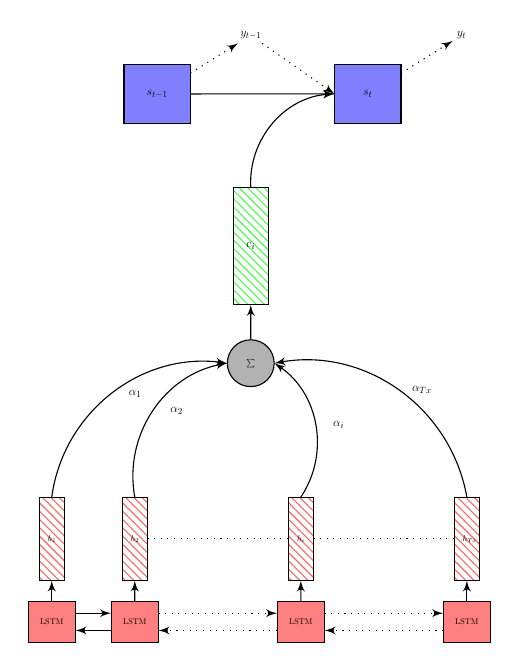
\begin{tikzpicture}[scale=0.3, every node/.style={transform shape}]
		\node[mlp_enc, node distance = 15em](LSTM_N_1){LSTM};
		\node[mlp_enc, right of=LSTM_N_1](LSTM_N_2) {LSTM};
		\path [line] (LSTM_N_1.20) to (LSTM_N_1.20-|LSTM_N_2.west);
		\path [line] (LSTM_N_2.200) to (LSTM_N_2.-20-|LSTM_N_1.east);     
		
		\node[mlp_enc, right of=LSTM_N_2, node distance = 20em](LSTM_N_i) {LSTM};
		\path [line, dotted] (LSTM_N_2.20) to (LSTM_N_2.20-|LSTM_N_i.west);
		\path [line, dotted] (LSTM_N_i.200) to (LSTM_N_i.200-|LSTM_N_2.east);
		
		\node[mlp_enc, right of=LSTM_N_i, node distance = 20em](LSTM_N_Tx) {LSTM};
		\path [line, dotted] (LSTM_N_i.20) to (LSTM_N_i.20-|LSTM_N_Tx.west);
		\path [line, dotted] (LSTM_N_Tx.200) to (LSTM_N_Tx.200-|LSTM_N_i.east);
		
		
		\node [enc_h, above of = LSTM_N_1] (h1) {$h_{1}$};
		\node [enc_h,above of = LSTM_N_2] (h2) {$h_{2}$};
		\node [enc_h,above of = LSTM_N_i] (hi) {$h_{i}$};
		\node [enc_h,above of = LSTM_N_Tx] (hTx) {$h_{Tx}$};
		
		\draw [dotted] (h2.east) to (hi.west);
		\draw [dotted] (hi.east) to (hTx.west);
		
		\path [line] (LSTM_N_1) to (h1);
		\path [line] (LSTM_N_2) to (h2);
		\path [line] (LSTM_N_i) to (hi);
		\path [line] (LSTM_N_Tx) to (hTx);
		
		
		\pause{}
		\fontsize{15}{12}
		\node [round, above of = h1, node distance = 15em, xshift=17em] (sum1) {$\sum$};
		
		\pause{}
		\path [line] (h1.north) to [bend left=45] node [xshift=2em] {$\alpha_{1}$} (sum1.west);
		\pause{}
		\path [line] (h2.north) to [bend left=45] node [xshift=2em] {$\alpha_{2}$} (sum1.west);
		\pause{}
		\path [line] (hi.north) to [bend right=45] node [xshift=2em] {$\alpha_{i}$} (sum1.east);
		\pause{}
		\path [line] (hTx.north) to [bend right=45] node [xshift=2em] {$\alpha_{Tx}$} (sum1.east);
		
		\pause{}
		\node [atts, above of = sum1] (ci) {$c_{i}$};
		
		\path [line] (sum1) to (ci.south);
		
		\pause{}
		\node [mlp_dec, above of = ci, xshift = -8em, yshift = 3em] (decoder_tm1) {$s_{t-1}$};
		\node [above of = decoder_tm1, node distance = 5em, xshift = 8em] (ytm1) {$y_{t-1}$};
		\path [line, dotted] (decoder_tm1) to (ytm1);
		\pause{}
		\pause{}
		\node [mlp_dec, right of = decoder_tm1, xshift = 8em] (decoder_t) {$s_{t}$};
		\path [line] (decoder_tm1.east) to (decoder_t.west);
		\path [line] (ci.north) to [bend left=45] (decoder_t.west);
		\path [line, dotted] (ytm1) to (decoder_t.west);
		\pause{}
		\node [above of = decoder_t, node distance = 5em, xshift = 8em] (yt) {$y_{t}$};
		\path [line, dotted] (decoder_t) to (yt);
		\end{tikzpicture}
	\end{center}
	\end{frame}
	
	\begin{frame}[fragile]{No Attention [Equal Attention?]}
	\begin{center}
		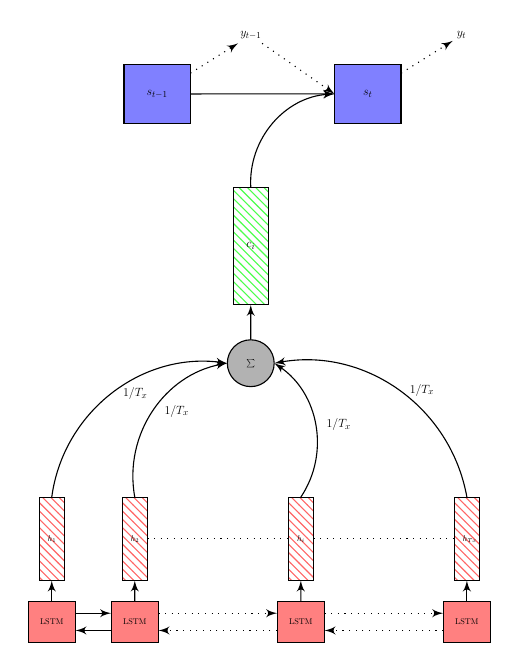
\begin{tikzpicture}[scale=0.3, every node/.style={transform shape}]
		\node[mlp_enc, node distance = 15em](LSTM_N_1){LSTM};
		\node[mlp_enc, right of=LSTM_N_1](LSTM_N_2) {LSTM};
		\path [line] (LSTM_N_1.20) to (LSTM_N_1.20-|LSTM_N_2.west);
		\path [line] (LSTM_N_2.200) to (LSTM_N_2.-20-|LSTM_N_1.east);     
		
		\node[mlp_enc, right of=LSTM_N_2, node distance = 20em](LSTM_N_i) {LSTM};
		\path [line, dotted] (LSTM_N_2.20) to (LSTM_N_2.20-|LSTM_N_i.west);
		\path [line, dotted] (LSTM_N_i.200) to (LSTM_N_i.200-|LSTM_N_2.east);
		
		\node[mlp_enc, right of=LSTM_N_i, node distance = 20em](LSTM_N_Tx) {LSTM};
		\path [line, dotted] (LSTM_N_i.20) to (LSTM_N_i.20-|LSTM_N_Tx.west);
		\path [line, dotted] (LSTM_N_Tx.200) to (LSTM_N_Tx.200-|LSTM_N_i.east);
		
		
		\node [enc_h, above of = LSTM_N_1] (h1) {$h_{1}$};
		\node [enc_h,above of = LSTM_N_2] (h2) {$h_{2}$};
		\node [enc_h,above of = LSTM_N_i] (hi) {$h_{i}$};
		\node [enc_h,above of = LSTM_N_Tx] (hTx) {$h_{Tx}$};
		
		\path [line] (LSTM_N_1) to (h1);
		\path [line] (LSTM_N_2) to (h2);
		\path [line] (LSTM_N_i) to (hi);
		\path [line] (LSTM_N_Tx) to (hTx);
		
		\draw [dotted] (h2.east) to (hi.west);
		\draw [dotted] (hi.east) to (hTx.west);
		
		
		\fontsize{15}{12}
		\node [round, above of = h1, node distance = 15em, xshift=17em] (sum1) {$\sum$};
		
		
		\path [line] (h1.north) to [bend left=45] node [xshift=2em] {$1/T_x$} (sum1.west);
		
		\path [line] (h2.north) to [bend left=45] node [xshift=2em] {$1/T_x$} (sum1.west);
		
		\path [line] (hi.north) to [bend right=45] node [xshift=2em] {$1/T_x$} (sum1.east);
		
		\path [line] (hTx.north) to [bend right=45] node [xshift=2em] {$1/T_x$} (sum1.east);
		
		
		\node [atts, above of = sum1] (ci) {$c_{i}$};
		
		\path [line] (sum1) to (ci.south);
		
		
		\node [mlp_dec, above of = ci, xshift = -8em, yshift = 3em] (decoder_tm1) {$s_{t-1}$};
		\node [above of = decoder_tm1, node distance = 5em, xshift = 8em] (ytm1) {$y_{t-1}$};
		\path [line, dotted] (decoder_tm1) to (ytm1);
		
		
		\node [mlp_dec, right of = decoder_tm1, xshift = 8em] (decoder_t) {$s_{t}$};
		\path [line] (decoder_tm1.east) to (decoder_t.west);
		\path [line] (ci.north) to [bend left=45] (decoder_t.west);
		\path [line, dotted] (ytm1) to (decoder_t.west);
		
		\node [above of = decoder_t, node distance = 5em, xshift = 8em] (yt) {$y_{t}$};
		\path [line, dotted] (decoder_t) to (yt);
		\end{tikzpicture}
	\end{center}
	\end{frame}
	
	\begin{frame}[fragile]{Dimensions of representations}
	\begin{center}
		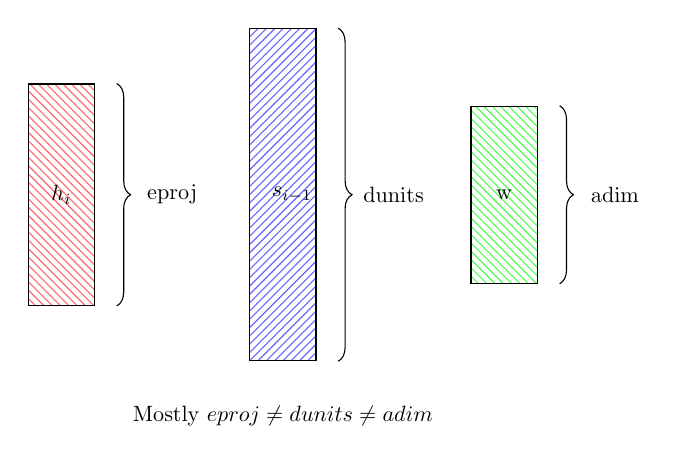
\begin{tikzpicture}[scale=0.8, every node/.style={transform shape}]
		\node [enc_h] (h1) {$h_{i}$};
		\draw [decorate,decoration={brace,amplitude=5pt, mirror, raise=2em}] (h1.south) -- (h1.north) node [black,midway,xshift=5em] {eproj};
		
		\node [dec_z, right of=h1, node distance = 10em, minimum height = 15em] (dec_z) {$s_{i-1}$};
		\draw [decorate,decoration={brace,amplitude=5pt, mirror, raise=2em}] (dec_z.south) -- (dec_z.north) node [black,midway,xshift=5em] {dunits};
		
		\node [atts, right of=dec_z, node distance = 10em, minimum height = 8em] (alpha) {w};
		\draw [decorate,decoration={brace,amplitude=5pt, mirror, raise=2em}] (alpha.south) -- (alpha.north) node [black,midway,xshift=5em] {adim};
		\node [below of=dec_z, node distance = 10em] {Mostly $ eproj \ne dunits \ne adim $};
		\end{tikzpicture}
	\end{center}
	\end{frame}

	\begin{frame}[fragile]{Matching the dimensions of representations}
	\begin{center}
		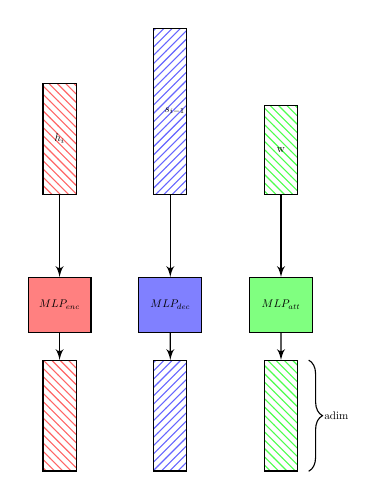
\begin{tikzpicture}[scale=0.4, every node/.style={transform shape}]
		\node [enc_h] (h1) {$h_{i}$};
		
		\node [dec_z, right of=h1, node distance = 10em, minimum height = 15em, yshift=2.5em] (dec_z) {$s_{i-1}$};
		
		\node [atts, right of=dec_z, node distance = 10em, minimum height = 8em, yshift=-3.5em] (alpha) {w};
		
		\node [mlp_enc, below of=h1, node distance = 15em] (mlp_enc) {$MLP_{enc}$};
		\node [mlp_dec, right of=mlp_enc, node distance = 10em] (mlp_dec) {$MLP_{dec}$};
		\node [mlp_att, right of=mlp_dec, node distance = 10em] (mlp_att) {$MLP_{att}$};
		
		\path [line] (h1.south) to (mlp_enc.north);
		\path [line] (dec_z.south) to (mlp_dec.north);
		\path [line] (alpha.south) to (mlp_att.north);
		
		\node [enc_h, below of=mlp_enc, node distance = 10em] (h_att) {};
		\node [dec_z, below of=mlp_dec, node distance = 10em] (z_att) {};
		\node [atts, below of=mlp_att, node distance = 10em] (alpha_att) {};
		
		\path [line] (mlp_enc.south) to (h_att.north);
		\path [line] (mlp_dec.south) to (z_att.north);
		\path [line] (mlp_att.south) to (alpha_att.north);
		\draw [decorate,decoration={brace,amplitude=5pt, mirror, raise=1em}] (alpha_att.south) -- (alpha_att.north) node [black,midway,xshift=5em] {adim};
		\end{tikzpicture}
	\end{center}
	\end{frame}

	\begin{frame}[fragile]{Dot product Attention}
	\begin{center}
		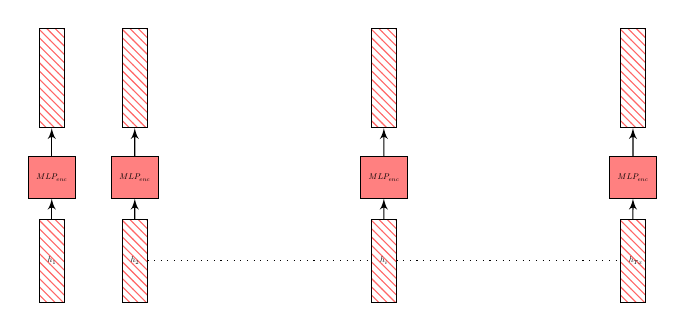
\begin{tikzpicture}[scale=0.3, every node/.style={transform shape}]
		\node [enc_h] (h1) {$h_{1}$};
		\node [enc_h,right of = h1] (h2) {$h_{2}$};
		\node [enc_h,right of = h2, node distance = 30em] (hi) {$h_{i}$};
		\node [enc_h,right of = hi, node distance = 30em] (hTx) {$h_{Tx}$};
		\draw [dotted] (h2.east) to (hi.west);
		\draw [dotted] (hi.east) to (hTx.west);
		\pause{}
		
		\node [mlp_enc, above of = h1, node distance = 10em] (mlp1) {$MLP_{enc}$};
		\path [line] (h1.north) to (mlp1.south);
		\node [enc_h, above of = mlp1, minimum height = 12em, node distance = 12em] (he1) {};
		\path [line] (mlp1.north) to (he1.south);
		
		\pause{}
		\node [mlp_enc, above of = h2, node distance = 10em] (mlp2) {$MLP_{enc}$};
		\path [line] (h2.north) to (mlp2.south);
		\node [enc_h, above of = mlp2, minimum height = 12em, node distance = 12em] (he2) {};
		\path [line] (mlp2.north) to (he2.south);
		
		\pause{}
		\node [mlp_enc, above of = hi, node distance = 10em] (mlpi) {$MLP_{enc}$};
		\path [line] (hi.north) to (mlpi.south);
		\node [enc_h, above of = mlpi, minimum height = 12em, node distance = 12em] (hei) {};
		\path [line] (mlpi.north) to (hei.south);
		
		\pause{}
		\node [mlp_enc, above of = hTx, node distance = 10em] (mlpTx) {$MLP_{enc}$};
		\path [line] (hTx.north) to (mlpTx.south);
		\node [enc_h, above of = mlpTx, minimum height = 12em, node distance = 12em] (heTx) {};
		\path [line] (mlpTx.north) to (heTx.south);
		\end{tikzpicture}
	\end{center}
	\end{frame}

	\begin{frame}[fragile]{Dot product Attention}
	\begin{center}
		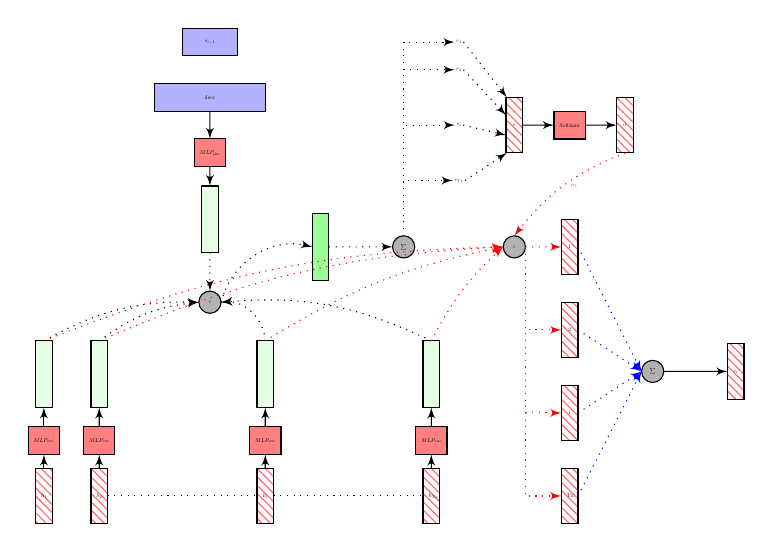
\begin{tikzpicture}[scale=0.2, every node/.style={transform shape}]
		\node [enc_h] (h1) {$h_{1}$};
		\node [enc_h,right of = h1] (h2) {$h_{2}$};
		\node [enc_h,right of = h2, node distance = 30em] (hi) {$h_{i}$};
		\node [enc_h,right of = hi, node distance = 30em] (hTx) {$h_{Tx}$};
		\draw [dotted] (h2.east) to (hi.west);
		\draw [dotted] (hi.east) to (hTx.west);
		
		
		\node [mlp_enc, above of = h1, node distance = 10em] (mlp1) {$MLP_{enc}$};
		\path [line] (h1.north) to (mlp1.south);
		\node [enc_h, above of = mlp1, minimum height = 12em, node distance = 12em, fill=green!10] (he1) {};
		\path [line] (mlp1.north) to (he1.south);
		
		
		\node [mlp_enc, above of = h2, node distance = 10em] (mlp2) {$MLP_{enc}$};
		\path [line] (h2.north) to (mlp2.south);
		\node [enc_h, above of = mlp2, minimum height = 12em, node distance = 12em, fill=green!10] (he2) {};
		\path [line] (mlp2.north) to (he2.south);
		
		
		\node [mlp_enc, above of = hi, node distance = 10em] (mlpi) {$MLP_{enc}$};
		\path [line] (hi.north) to (mlpi.south);
		\node [enc_h, above of = mlpi, minimum height = 12em, node distance = 12em, fill=green!10] (hei) {};
		\path [line] (mlpi.north) to (hei.south);
		
		
		\node [mlp_enc, above of = hTx, node distance = 10em] (mlpTx) {$MLP_{enc}$};
		\path [line] (hTx.north) to (mlpTx.south);
		\node [enc_h, above of = mlpTx, minimum height = 12em, node distance = 12em, fill=green!10] (heTx) {};
		\path [line] (mlpTx.north) to (heTx.south);
		
		\node [mlp_enc, fill=blue!30, above of = hei, node distance = 60em, minimum width = 10em, xshift = -10em] (sim1) {$s_{i-1}$};
		\node [mlp_enc, fill=blue!30 , below of=sim1, minimum width = 20em] (dec_z) {decz};
		\node [mlp_enc, below of=dec_z, node distance = 10em] (mlp_dec) {$MLP_{dec}$};
		\path [line] (dec_z) to (mlp_dec);
		\node [enc_h, below of = mlp_dec, minimum height = 12em, node distance = 12em, fill=green!10] (decz_enc) {};
		\path [line] (mlp_dec) to (decz_enc);
		
		\node [round, below of = decz_enc, node distance = 15em] (prod) {$\circ$}; 
		
		\pause{}
		\path [line, dotted] (he1.north) to [bend left=15] (prod.west);
		\path [line, dotted] (decz_enc.south) to (prod.north);
		
		\node [enc_h, right of = prod, minimum height = 12em, node distance = 20em, yshift=10em, fill=green!40] (h_z) {};
		\path [line, dotted] (prod.east) to [bend left=45] (h_z.west);
		
		\pause{}
		\node [round, right of = h_z, node distance = 15em] (sum) {$\sum$};
		\path [line, dotted] (h_z.east) to (sum.west);
		
		\pause{}
		\node [right of=sim1, node distance = 15em, xshift=30em] (e1) {$e_{1}$};
		\path [line, dotted] (sum.north) |- (e1.west);
		
		\pause{}
		\node [below of=e1, node distance = 5em] (e2) {$e_{2}$};
		\path [line, dotted] (he2.north) to [bend left=15] (prod.west);
		\path [line, dotted] (sum.north) |- (e2.west);
		
		\pause{}
		\node [below of=e2, node distance = 10em] (ei) {$e_{i}$};
		\path [line, dotted] (hei.north) to [bend right=45] (prod.east);
		\path [line, dotted] (sum.north) |- (ei.west);
		
		\pause{}
		\node [below of=ei, node distance = 10em] (eTx) {$e_{Tx}$};
		\path [line, dotted] (heTx.north) to [bend right=15] (prod.east);
		\path [line, dotted] (sum.north) |- (eTx.west);
		
		\pause{}
		\node [enc_h, right of=ei] (e) {e};
		
		\pause{}
		\path [line, dotted] (e1.east) to (e.105);
		\path [line, dotted] (e2.east) to (e.130);
		\path [line, dotted] (ei.east) to (e.-130);
		\path [line, dotted] (eTx.east) to (e.-105);
		
		\pause{}
		\node [mlp_enc, right of=e] (sm) {Softmax};
		\path [line] (e.east) to (sm.west);
		
		\pause{}
		\node [enc_h, right of=sm] (alphas) {$\alpha$};
		\path [line] (sm.east) to (alphas.west);
		
		\pause{}
		\node [round, right of=sum, node distance=20em] (alpha_h) {$\circ$};
		\path [line, dotted, color=red] (he1.north) to [bend left=10] (alpha_h.west);
		\path [line, dotted, color=red] (alphas.south) to [bend right=15] node [xshift=2em] {$\alpha_{1}$} (alpha_h.north);
		
		\pause{}
		\node [enc_h, right of=alpha_h] (ahe1) {1};
		\path [line, dotted, color=red] (alpha_h.east) to (ahe1.west);
		
		\pause{}
		\path [line, dotted, color=red] (he2.north) to [bend left=10] (alpha_h.west);
		\node [enc_h, below of=ahe1, node distance = 15em] (ahe2) {2};
		\path [line, dotted, color=red] (alpha_h.east) |- (ahe2.west);
		
		\pause{}
		\path [line, dotted, color=red] (hei.north) to [bend left=10] (alpha_h.west);
		\node [enc_h, below of=ahe2, node distance = 15em] (ahei) {i};
		\path [line, dotted, color=red] (alpha_h.east) |- (ahei.west);
		
		\pause{}
		\path [line, dotted, color=red] (heTx.north) to [bend left=10] (alpha_h.west);
		\node [enc_h, below of=ahei, node distance = 15em] (aheTx) {Tx};
		\path [line, dotted, color=red] (alpha_h.east) |- (aheTx.west);
		
		\pause{}
		\node [round, right of=ahe2, yshift=-7.5em, node distance = 15em] (sum_op) {$\sum$};
		\path [line, dotted, color=blue] (ahe1.east) to (sum_op.west);
		\path [line, dotted, color=blue] (ahe2.east) to (sum_op.west);
		\path [line, dotted, color=blue] (ahei.east) to (sum_op.west);
		\path [line, dotted, color=blue] (aheTx.east) to (sum_op.west);
		
		\pause{}
		\node [enc_h, right of=sum_op, node distance=15em] (ci) {$c_i$};
		\path [line] (sum_op.east) to (ci.west);
		\end{tikzpicture}
	\end{center}
	\end{frame}
\section{First}
\section{Second}
\section{Third}

\end{document}
